\section{Background}
\label{sec:background}

Evolutionary Algorithms (EAs) are widely used for solving black-box optimization problems, drawing inspiration from Darwinian evolution. These algorithms operate by evolving a population of solutions through the mechanisms of selection, recombination, and mutation like for example in Genetic Algorithms (GAs) \cite{holland_ga_1992} or Evolution Strategies (ES) \cite{back_es_1996}. However, like their biological inspiration, mutation and recombination in EAs are random processes and only selection is deterministic. This randomness implies that the algorithm does not explicitly take into account the correlation between different parts of the genotype and its impact on the fitness landscape and the process is only guided by selection pressure. Consequently, the search process may be inefficient or flat out wrong in navigating deceptive fitness landscapes. If this correlation were explicitly modeled, it could potentially lead to more effective search processes.

In contrast to traditional EAs, Estimation of Distribution Algorithms (EDAs) \cite{larranaga_estimation_2002} represent a class of algorithms that aim to improve search efficiency by modeling the distribution of the best solutions discovered so far. EDAs construct a probabilistic model of the population, which is then used to generate new candidate solutions (Figure \ref{fig:eda}). By sampling from this model and selecting the best candidates, the search is guided towards more promising areas of the search space. The complexity of the dependencies modelled by the probabilistic model used can vary depending on the complexity of the optimization problem and the available computational resources. Most simple EDAs assume that the $n$-dimensional joint probability factorizes into the product of $n$ univariate distributions like in Univariate Marginal Distribution Algorithm (UMDA) \cite{muhlenbein_umda_1997}. A common approach to model more complex dependencies is to use Probabilistic Graphical Models (PGMs) like Bayesian Networks. For example Estimation of Bayesian Networks Algorithm (EBNA) \cite{larranaga_ebna_2000} constructs a Bayesian Network to model the population starting from an edge-less graph and adding edges based on some statistical test while Bayesian Optimization Algorithm (BOA) \cite{pelikan_boa_2005} uses the Bayesian-Dirichlet metric to compare the score of Bayesian Networks that encode the same conditional independency relationships.

\begin{figure}
    \centering
    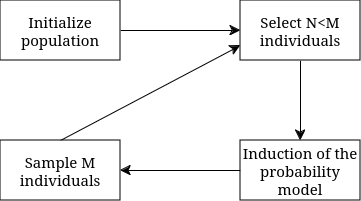
\includegraphics[width=0.3\textwidth]{img/eda.png}
    \caption{Estimation of Distribution Algorithm (EDA)}
    \label{fig:eda}
\end{figure}

Another possible approach is to use Markov Networks to model the dependencies between variables \cite{shakya_markov_2012}. A Markov Networks is a type of probabilistic graphical model represented as a pair $(G, \Psi)$, where $G$ is an undirected graph and $\Psi$ is the parameter set of the model. Unlike the more common Bayesian Networks, Markov Networks are undirected PGM and thus do make any assumption about the direction of the dependencies between variables (and thus do not have a notion of causality). While this allows to factorize a broader class of probability distributions\footnote{Note, however, that there are probability distributions that can be modelled by Bayesian Networks but not Markov Networks.}, it also makes the structure and parameter learning as well as inference more complex.

A Markov Network is characterized by two key properties:
\begin{enumerate}
    \item \textit{Local Markov property (Markovianity)}: A variable is conditionally independent of all other variables, given its neighbors (also known as the Markov blanket).
          \begin{equation*}
              P(x_i | x - \{x_i\}) = P(x_i | x_{\text{ne}(i)})
          \end{equation*}

    \item \textit{Global Markov property}: the joint probability distribution can be factorized as the product of the potential functions defined over the cliques of the graph.
          \begin{align*}
              P(x) & = \frac{1}{Z} \prod_{i=1}^m \psi_i(c_i) = \frac{1}{\sum_{x \in \Omega} \prod_{i=1}^m \psi_i(c_i)} \prod_{i=1}^m \psi_i(c_i) \\
          \end{align*}
          where $Z$, the partition function, is a normalization constant and usually intractable to compute. Equivalently, the joint distribution can be expressed using a Gibbs/Boltzmann distribution:
          \begin{equation*}
              P(x) = \frac{1}{Z} e^{-U(x)/T} = \frac{1}{\sum_{y \in \Omega} e^{-U(y)/T}} e^{-U(x)/T}
          \end{equation*}
          Here, $T$ is the temperature, and $U(x)=\sum_{i=1}^m u_i(c_i)$ represents the energy of the distribution.
\end{enumerate}

Both the local and global property can be exploited to model the population in an EDA. For example, in Markovianity based Optimization Algorithm (MOA) \cite{shakya_moa_2011} Shakya et al. first estimate the structure of the network by computing mutual information between every pair of variables. Then, by exploiting the local Markov property, they can directly sample from the underlying distribution without the need to perform parameter estimation.

On the other hand, Distribution Estimation using Markov Random Fields (DEUM) \cite{shakya_deum_2012} first estimates the network structure using statistical tests to determine the independency relationships between variables, then they try to learn the parameters so as to increase the probability of the best solutions in the population. Since naive parameter estimation would require to compute the partition function, they assume that each solution in the search space has a probability proportional to its fitness:

\begin{equation*}
    p(x) = \frac{f(x)}{Z} = \frac{f(x)}{\sum_{y \in \Omega} f(y)}
\end{equation*}

Then, by exploiting the global Markov property and equating the empirical density of a solution to the one of the model, they show that fitting the parameters of the model can be transformed into a simple regression problem:

\begin{align*}
    p(x) = \frac{f(x)}{\sum_{y \in \Omega} f(y)} & = \frac{e^{-U(x)/T}}{\sum_{y \in \Omega} e^{-U(y)/T}} \\
    -\log f(x)                                   & = U(x)
\end{align*}

Besides expressing the joint probability distribution of Markov Networks, the Boltzmann distribution is also the foundation of energy-based models \cite{teh_ebm_2003}, which are a class of models that define a probability distribution over the data by assigning an energy $E(x)$ to each configuration $x$.
\begin{equation*}
    p(x) = \frac{1}{Z_{\theta}} e^{-\beta E_{\theta}(x)}
\end{equation*}
This approach offers great flexibility, as any function (e.g., a neural network) can be used to model the energy of the distribution. However, a significant challenge arises from the normalization constant $Z_{\theta} = \int_{x \in X} -e^{-\beta E_{\theta}(x)} dx$, which is usually intractable. The standard method for learning a probabilistic model $p_{\theta}(x)$ is to maximize the expected log-likelihood of the data \cite{song_ebm_2021}:
\begin{equation}
    \mathcal{L}(\theta) = \mathbb{E}_{x \sim p_{\text{data}}(x)}[\log p_{\theta}(x)]
\end{equation}
Because of the intractability of the normalization constant, the expected log-likelihood is usually approximated using Markov Chain Monte Carlo (MCMC) approaches. One of the most widely used MCMC methods is Langevin dynamics \cite{parisi_langevin_1980}, which leverages the fact that the gradient of the log-probability is equal to the negative gradient of the energy:
\begin{align*}
    x_{t+1} & = x_t + \frac{\epsilon}{2} \nabla E(x_t) + \sqrt{2 \epsilon} z_i                  \\
            & = x_t - \frac{\epsilon}{2} \nabla \log p(x) + \sqrt{2 \epsilon} \mathcal{N}(0, I)
\end{align*}
